\documentclass[]{article}
\usepackage{lmodern}
\usepackage{amssymb,amsmath}
\usepackage{ifxetex,ifluatex}
\usepackage{fixltx2e} % provides \textsubscript
\ifnum 0\ifxetex 1\fi\ifluatex 1\fi=0 % if pdftex
  \usepackage[T1]{fontenc}
  \usepackage[utf8]{inputenc}
\else % if luatex or xelatex
  \ifxetex
    \usepackage{mathspec}
  \else
    \usepackage{fontspec}
  \fi
  \defaultfontfeatures{Ligatures=TeX,Scale=MatchLowercase}
\fi
% use upquote if available, for straight quotes in verbatim environments
\IfFileExists{upquote.sty}{\usepackage{upquote}}{}
% use microtype if available
\IfFileExists{microtype.sty}{%
\usepackage{microtype}
\UseMicrotypeSet[protrusion]{basicmath} % disable protrusion for tt fonts
}{}
\usepackage[margin=1in]{geometry}
\usepackage{hyperref}
\hypersetup{unicode=true,
            pdftitle={Spectral Graph Clustering using gmmase},
            pdfauthor={JHU Team},
            pdfborder={0 0 0},
            breaklinks=true}
\urlstyle{same}  % don't use monospace font for urls
\usepackage{color}
\usepackage{fancyvrb}
\newcommand{\VerbBar}{|}
\newcommand{\VERB}{\Verb[commandchars=\\\{\}]}
\DefineVerbatimEnvironment{Highlighting}{Verbatim}{commandchars=\\\{\}}
% Add ',fontsize=\small' for more characters per line
\usepackage{framed}
\definecolor{shadecolor}{RGB}{248,248,248}
\newenvironment{Shaded}{\begin{snugshade}}{\end{snugshade}}
\newcommand{\KeywordTok}[1]{\textcolor[rgb]{0.13,0.29,0.53}{\textbf{#1}}}
\newcommand{\DataTypeTok}[1]{\textcolor[rgb]{0.13,0.29,0.53}{#1}}
\newcommand{\DecValTok}[1]{\textcolor[rgb]{0.00,0.00,0.81}{#1}}
\newcommand{\BaseNTok}[1]{\textcolor[rgb]{0.00,0.00,0.81}{#1}}
\newcommand{\FloatTok}[1]{\textcolor[rgb]{0.00,0.00,0.81}{#1}}
\newcommand{\ConstantTok}[1]{\textcolor[rgb]{0.00,0.00,0.00}{#1}}
\newcommand{\CharTok}[1]{\textcolor[rgb]{0.31,0.60,0.02}{#1}}
\newcommand{\SpecialCharTok}[1]{\textcolor[rgb]{0.00,0.00,0.00}{#1}}
\newcommand{\StringTok}[1]{\textcolor[rgb]{0.31,0.60,0.02}{#1}}
\newcommand{\VerbatimStringTok}[1]{\textcolor[rgb]{0.31,0.60,0.02}{#1}}
\newcommand{\SpecialStringTok}[1]{\textcolor[rgb]{0.31,0.60,0.02}{#1}}
\newcommand{\ImportTok}[1]{#1}
\newcommand{\CommentTok}[1]{\textcolor[rgb]{0.56,0.35,0.01}{\textit{#1}}}
\newcommand{\DocumentationTok}[1]{\textcolor[rgb]{0.56,0.35,0.01}{\textbf{\textit{#1}}}}
\newcommand{\AnnotationTok}[1]{\textcolor[rgb]{0.56,0.35,0.01}{\textbf{\textit{#1}}}}
\newcommand{\CommentVarTok}[1]{\textcolor[rgb]{0.56,0.35,0.01}{\textbf{\textit{#1}}}}
\newcommand{\OtherTok}[1]{\textcolor[rgb]{0.56,0.35,0.01}{#1}}
\newcommand{\FunctionTok}[1]{\textcolor[rgb]{0.00,0.00,0.00}{#1}}
\newcommand{\VariableTok}[1]{\textcolor[rgb]{0.00,0.00,0.00}{#1}}
\newcommand{\ControlFlowTok}[1]{\textcolor[rgb]{0.13,0.29,0.53}{\textbf{#1}}}
\newcommand{\OperatorTok}[1]{\textcolor[rgb]{0.81,0.36,0.00}{\textbf{#1}}}
\newcommand{\BuiltInTok}[1]{#1}
\newcommand{\ExtensionTok}[1]{#1}
\newcommand{\PreprocessorTok}[1]{\textcolor[rgb]{0.56,0.35,0.01}{\textit{#1}}}
\newcommand{\AttributeTok}[1]{\textcolor[rgb]{0.77,0.63,0.00}{#1}}
\newcommand{\RegionMarkerTok}[1]{#1}
\newcommand{\InformationTok}[1]{\textcolor[rgb]{0.56,0.35,0.01}{\textbf{\textit{#1}}}}
\newcommand{\WarningTok}[1]{\textcolor[rgb]{0.56,0.35,0.01}{\textbf{\textit{#1}}}}
\newcommand{\AlertTok}[1]{\textcolor[rgb]{0.94,0.16,0.16}{#1}}
\newcommand{\ErrorTok}[1]{\textcolor[rgb]{0.64,0.00,0.00}{\textbf{#1}}}
\newcommand{\NormalTok}[1]{#1}
\usepackage{longtable,booktabs}
\usepackage{graphicx,grffile}
\makeatletter
\def\maxwidth{\ifdim\Gin@nat@width>\linewidth\linewidth\else\Gin@nat@width\fi}
\def\maxheight{\ifdim\Gin@nat@height>\textheight\textheight\else\Gin@nat@height\fi}
\makeatother
% Scale images if necessary, so that they will not overflow the page
% margins by default, and it is still possible to overwrite the defaults
% using explicit options in \includegraphics[width, height, ...]{}
\setkeys{Gin}{width=\maxwidth,height=\maxheight,keepaspectratio}
\IfFileExists{parskip.sty}{%
\usepackage{parskip}
}{% else
\setlength{\parindent}{0pt}
\setlength{\parskip}{6pt plus 2pt minus 1pt}
}
\setlength{\emergencystretch}{3em}  % prevent overfull lines
\providecommand{\tightlist}{%
  \setlength{\itemsep}{0pt}\setlength{\parskip}{0pt}}
\setcounter{secnumdepth}{5}
% Redefines (sub)paragraphs to behave more like sections
\ifx\paragraph\undefined\else
\let\oldparagraph\paragraph
\renewcommand{\paragraph}[1]{\oldparagraph{#1}\mbox{}}
\fi
\ifx\subparagraph\undefined\else
\let\oldsubparagraph\subparagraph
\renewcommand{\subparagraph}[1]{\oldsubparagraph{#1}\mbox{}}
\fi

%%% Use protect on footnotes to avoid problems with footnotes in titles
\let\rmarkdownfootnote\footnote%
\def\footnote{\protect\rmarkdownfootnote}

%%% Change title format to be more compact
\usepackage{titling}

% Create subtitle command for use in maketitle
\newcommand{\subtitle}[1]{
  \posttitle{
    \begin{center}\large#1\end{center}
    }
}

\setlength{\droptitle}{-2em}
  \title{Spectral Graph Clustering using \texttt{gmmase}}
  \pretitle{\vspace{\droptitle}\centering\huge}
  \posttitle{\par}
  \author{JHU Team}
  \preauthor{\centering\large\emph}
  \postauthor{\par}
  \predate{\centering\large\emph}
  \postdate{\par}
  \date{2017-09-17}


\begin{document}
\maketitle

{
\setcounter{tocdepth}{2}
\tableofcontents
}
Given a (possibly directed) (possibly weighted) graph \(G=(V,E)\), the
\texttt{gmmase} package does

\begin{enumerate}
\def\labelenumi{\arabic{enumi}.}
\tightlist
\item
  do a \emph{pass-to-rank} for a weighted graph (\texttt{PTR}, no-op for
  an unweighted graph),
\item
  do a \emph{graph spectral embedding} (\texttt{ASE} or
  \texttt{LSE}\footnote{D.L. Sussman, M. Tang, D.E. Fishkind, and C.E.
    Priebe, A consistent adjacency spectral embedding for stochastic
    blockmodel graphs, Journal of the American Statistical Association,
    Vol. 107, No. 499, pp.~1119-1128, 2012.}) with a \emph{diagonal
  augmentation},
\item
  do a \emph{dimension reduction} (\texttt{ZG}\footnote{M. Zhu, and A.
    Ghodsi, Automatic dimensionality selection from the scree plot via
    the use of profile likelihood. Computational Statistics and Data
    Analysis, Vol. 51, 918--930, 2006.}) and merge left and right
  vectors (no-op for an undirected graph),
\item
  cluster vertices (\texttt{GMM}\footnote{MCLUST Version 4 for R: Normal
    Mixture Modeling for Model-Based Clustering, Classification, and
    Density Estimation, Technical Report no. 597, Department of
    Statistics, University of Washington, June 2012.} or
  \texttt{Kmeans}).
\end{enumerate}

\section{Connectome Data}\label{connectome-data}

This vignette demo uses a connectome data\footnote{K. Eichler, F. Li, A.
  L. Kumar, Y. Park, I. Andrade, C. Schneider-Mizell, T. Saumweber, A.
  Huser, D. Bonnery, B. Gerber, R. D. Fetter, J. W. Truman, C. E.
  Priebe, L. F. Abbott, A. Thum, M. Zlatic, and A. Cardona, ``The
  complete connectome of a learning and memory center in an insect
  brain,'' Nature, no. 548, pp.~175-182, 2017.} with 123 vertices and
2740 edges.

\begin{Shaded}
\begin{Highlighting}[]
\KeywordTok{library}\NormalTok{(gmmase)}
\KeywordTok{suppressPackageStartupMessages}\NormalTok{(}\KeywordTok{library}\NormalTok{(igraph))}

\KeywordTok{data}\NormalTok{(}\StringTok{"akira"}\NormalTok{)}
\KeywordTok{summary}\NormalTok{(akira)}
\end{Highlighting}
\end{Shaded}

\begin{verbatim}
# IGRAPH 1770d3c DNW- 123 2740 -- 
# + attr: name (v/c), weight (e/n)
\end{verbatim}

\begin{Shaded}
\begin{Highlighting}[]
\NormalTok{knitr}\OperatorTok{::}\KeywordTok{kable}\NormalTok{(}\KeywordTok{as.matrix}\NormalTok{(akira[])[}\DecValTok{1}\OperatorTok{:}\DecValTok{10}\NormalTok{,}\DecValTok{1}\OperatorTok{:}\DecValTok{10}\NormalTok{], }\DataTypeTok{digits=}\DecValTok{2}\NormalTok{)}
\end{Highlighting}
\end{Shaded}

\begin{longtable}[]{@{}lrrrrrrrrrr@{}}
\toprule
& CN1\_FB5 & CN2 & CN3 & CN4\_FB12 & CN5\_FB13 & CN6\_FB16 & CN7 &
CN8\_FB21 & CN9 & CN10\tabularnewline
\midrule
\endhead
CN1\_FB5 & 0.00 & 0.00 & 0.00 & 0.00 & 0.00 & 0.00 & 0.19 & 0 & 0 &
0\tabularnewline
CN2 & 0.00 & 0.00 & 0.28 & 0.21 & 0.00 & 0.00 & 0.00 & 0 & 0 &
0\tabularnewline
CN3 & 0.00 & 0.25 & 0.00 & 0.10 & 0.23 & 0.10 & 0.00 & 0 & 0 &
0\tabularnewline
CN4\_FB12 & 0.00 & 0.00 & 0.00 & 0.00 & 0.00 & 0.00 & 0.00 & 0 & 0 &
0\tabularnewline
CN5\_FB13 & 0.00 & 0.00 & 0.00 & 0.00 & 0.00 & 0.31 & 0.00 & 0 & 0 &
0\tabularnewline
CN6\_FB16 & 0.00 & 0.00 & 0.00 & 0.00 & 0.80 & 0.00 & 0.00 & 0 & 0 &
0\tabularnewline
CN7 & 0.00 & 0.00 & 0.00 & 0.00 & 0.00 & 0.00 & 0.00 & 0 & 0 &
0\tabularnewline
CN8\_FB21 & 0.00 & 0.06 & 0.14 & 0.00 & 0.00 & 0.10 & 0.00 & 0 & 0 &
0\tabularnewline
CN9 & 0.00 & 0.00 & 0.00 & 0.00 & 0.00 & 0.00 & 0.00 & 0 & 0 &
0\tabularnewline
CN10 & 0.13 & 0.81 & 0.00 & 0.00 & 1.48 & 2.28 & 0.00 & 0 & 0 &
0\tabularnewline
\bottomrule
\end{longtable}

\begin{Shaded}
\begin{Highlighting}[]
\CommentTok{# take induced subgraph using only CN neurons}
\NormalTok{cn <-}\StringTok{ }\KeywordTok{grep}\NormalTok{(}\StringTok{"CN"}\NormalTok{, }\KeywordTok{V}\NormalTok{(akira)}\OperatorTok{$}\NormalTok{name)}
\NormalTok{g.cn <-}\StringTok{ }\KeywordTok{induced_subgraph}\NormalTok{(akira, cn)}
\end{Highlighting}
\end{Shaded}

\subsection{\texorpdfstring{\texttt{gmmase}}{gmmase}}\label{gmmase}

\begin{Shaded}
\begin{Highlighting}[]
\NormalTok{out <-}\StringTok{ }\KeywordTok{gmmase}\NormalTok{(g.cn, }\DataTypeTok{dmax =} \DecValTok{20}\NormalTok{, }\DataTypeTok{embed =} \StringTok{"ASE"}\NormalTok{, }\DataTypeTok{clustering =} \StringTok{"GMM"}\NormalTok{, }\DataTypeTok{verbose=}\OtherTok{FALSE}\NormalTok{)}
\end{Highlighting}
\end{Shaded}

\begin{verbatim}
# 1. Finding an lcc...
# IGRAPH fd4bbd3 DNW- 43 515 -- 
# + attr: name (v/c), weight (e/n)
# 2. Passing-to-rank...
# IGRAPH fd4bbd3 DNW- 43 515 -- 
# + attr: name (v/c), weight (e/n)
# 3. Embedding the graph into dmax = 20...
# 4. Finding an elbow (dimension reduction)..., use dhat =  2 
# 5. Clustering vertices..., Khat =  4 
# ----------------------------------------------------
# Gaussian finite mixture model fitted by EM algorithm 
# ----------------------------------------------------
# 
# Mclust EEV (ellipsoidal, equal volume and shape) model with 4 components:
# 
#  log.likelihood  n df       BIC       ICL
#        74.86953 43 47 -27.03735 -27.88816
# 
# Clustering table:
#  1  2  3  4 
# 11  8  9 15
\end{verbatim}

Now, we are plotting a paired scatter plot colored by the clustering
labels.

\begin{Shaded}
\begin{Highlighting}[]
\NormalTok{g <-}\StringTok{ }\NormalTok{out}\OperatorTok{$}\NormalTok{g}
\NormalTok{mc <-}\StringTok{ }\NormalTok{out}\OperatorTok{$}\NormalTok{mc}
\NormalTok{Xhat <-}\StringTok{ }\NormalTok{mc}\OperatorTok{$}\NormalTok{data}
\NormalTok{dhat <-}\StringTok{ }\KeywordTok{ncol}\NormalTok{(Xhat)}\OperatorTok{/}\DecValTok{2}
\NormalTok{Khat <-}\StringTok{ }\NormalTok{mc}\OperatorTok{$}\NormalTok{G}
\KeywordTok{colnames}\NormalTok{(Xhat) <-}\StringTok{ }\KeywordTok{paste0}\NormalTok{(}\KeywordTok{rep}\NormalTok{(}\KeywordTok{c}\NormalTok{(}\StringTok{"out"}\NormalTok{,}\StringTok{"in"}\NormalTok{),}\DataTypeTok{each=}\DecValTok{2}\NormalTok{), }\DecValTok{1}\OperatorTok{:}\DecValTok{2}\NormalTok{)}
\NormalTok{class <-}\StringTok{ }\NormalTok{mc}\OperatorTok{$}\NormalTok{classification}
\NormalTok{df <-}\StringTok{ }\KeywordTok{data.frame}\NormalTok{(Xhat, }\DataTypeTok{cluster=}\KeywordTok{factor}\NormalTok{(class))}

\KeywordTok{library}\NormalTok{(ggplot2)}
\KeywordTok{library}\NormalTok{(GGally)}
\end{Highlighting}
\end{Shaded}

\begin{verbatim}
# 
# Attaching package: 'GGally'
\end{verbatim}

\begin{verbatim}
# The following object is masked from 'package:dplyr':
# 
#     nasa
\end{verbatim}

\begin{Shaded}
\begin{Highlighting}[]
\KeywordTok{ggpairs}\NormalTok{(df, }\DataTypeTok{columns=}\DecValTok{1}\OperatorTok{:}\KeywordTok{ncol}\NormalTok{(Xhat), }\DataTypeTok{mapping=}\KeywordTok{aes}\NormalTok{(}\DataTypeTok{color=}\NormalTok{cluster, }\DataTypeTok{alpha=}\FloatTok{0.5}\NormalTok{))}
\end{Highlighting}
\end{Shaded}

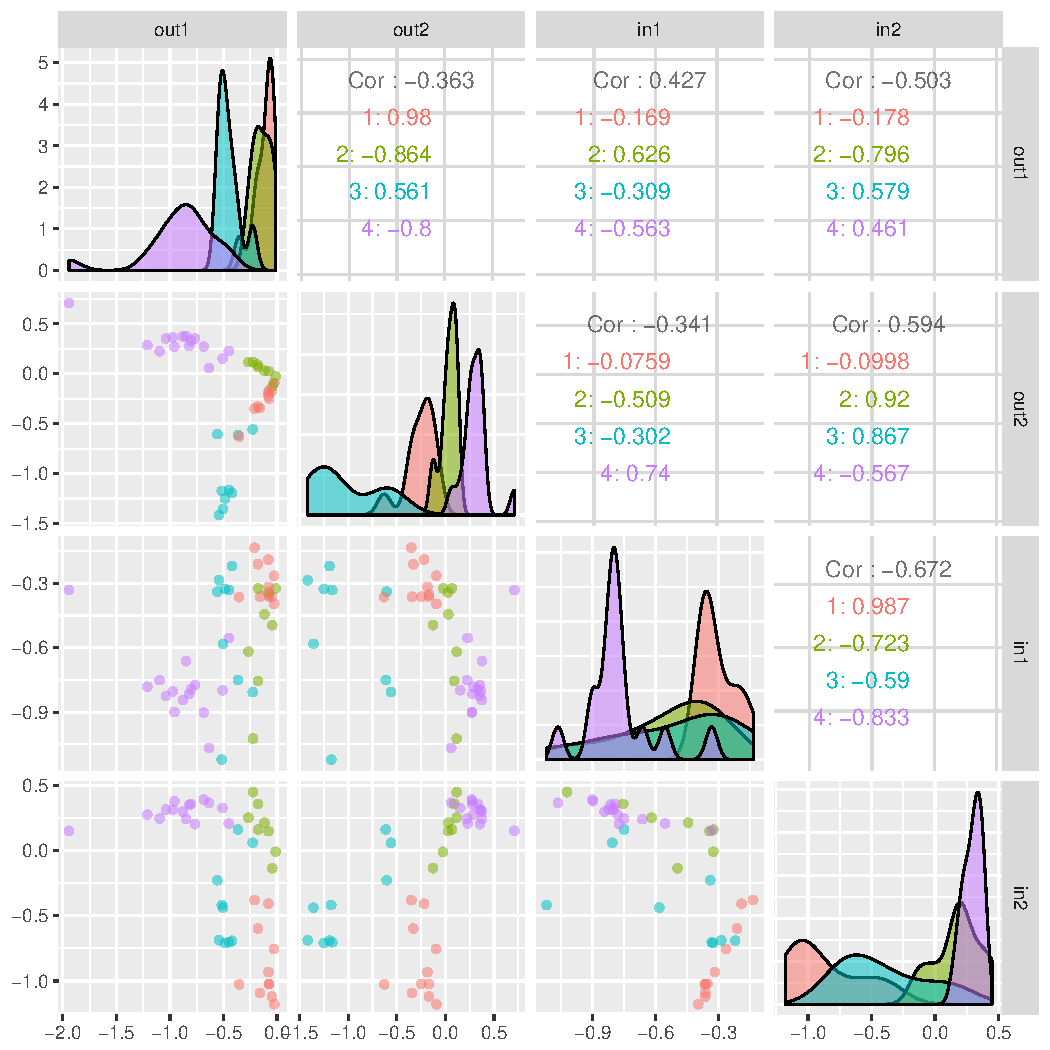
\includegraphics{gmmase_files/figure-latex/post-1.pdf}

\subsection{co-clustering}\label{co-clustering}

The data provider informed us from their beahvioral experiments that
following neurons should be clustered onto their own groups.

\begin{itemize}
\tightlist
\item
  \texttt{CN4}, \texttt{CN12} \texttt{CN18}, and \texttt{CN41},
\item
  \texttt{CN19},
\item
  \texttt{CN40}.
\end{itemize}

\begin{Shaded}
\begin{Highlighting}[]
\NormalTok{v1 <-}\StringTok{ }\KeywordTok{c}\NormalTok{(}\DecValTok{4}\NormalTok{,}\DecValTok{12}\NormalTok{,}\DecValTok{18}\NormalTok{,}\DecValTok{41}\NormalTok{)}
\NormalTok{v2 <-}\StringTok{ }\DecValTok{40}
\NormalTok{v3 <-}\StringTok{ }\DecValTok{19}
\NormalTok{vcc<-}\StringTok{ }\KeywordTok{c}\NormalTok{(v1,v2,v3)}
\NormalTok{df2 <-}\StringTok{ }\KeywordTok{data.frame}\NormalTok{(}\DataTypeTok{name=}\KeywordTok{V}\NormalTok{(g)}\OperatorTok{$}\NormalTok{name, }\DataTypeTok{cluster=}\NormalTok{class)}
\NormalTok{df2[vcc,]}
\end{Highlighting}
\end{Shaded}

\begin{verbatim}
#           name cluster
# 4     CN4_FB12       1
# 12   CN12_FB25       1
# 18   CN18_FB30       1
# 41 MBONm1_CN41       1
# 40 MBONc1_CN40       4
# 19        CN19       2
\end{verbatim}

\begin{Shaded}
\begin{Highlighting}[]
\KeywordTok{V}\NormalTok{(g)}\OperatorTok{$}\NormalTok{color <-}\StringTok{ "orange"}
\KeywordTok{V}\NormalTok{(g)}\OperatorTok{$}\NormalTok{color[v1] <-}\StringTok{ "magenta"}
\KeywordTok{V}\NormalTok{(g)}\OperatorTok{$}\NormalTok{color[v2] <-}\StringTok{ "cyan"}
\KeywordTok{V}\NormalTok{(g)}\OperatorTok{$}\NormalTok{color[v3] <-}\StringTok{ "green"}

\KeywordTok{plot}\NormalTok{(g, }\DataTypeTok{mark.groups=}\KeywordTok{lapply}\NormalTok{(}\DecValTok{1}\OperatorTok{:}\NormalTok{Khat, }\ControlFlowTok{function}\NormalTok{(x) }\KeywordTok{which}\NormalTok{(class}\OperatorTok{==}\NormalTok{x)),}
     \DataTypeTok{edge.arrow.size=}\FloatTok{0.5}\NormalTok{, }\DataTypeTok{vertex.label=}\OtherTok{NA}\NormalTok{, }\CommentTok{#vertex.label.cex=0.8, }
     \DataTypeTok{vertex.size=}\DecValTok{7}\NormalTok{)}\CommentTok{#, vertex.color=rainbow(3, alpha=.5)[class])}
\end{Highlighting}
\end{Shaded}

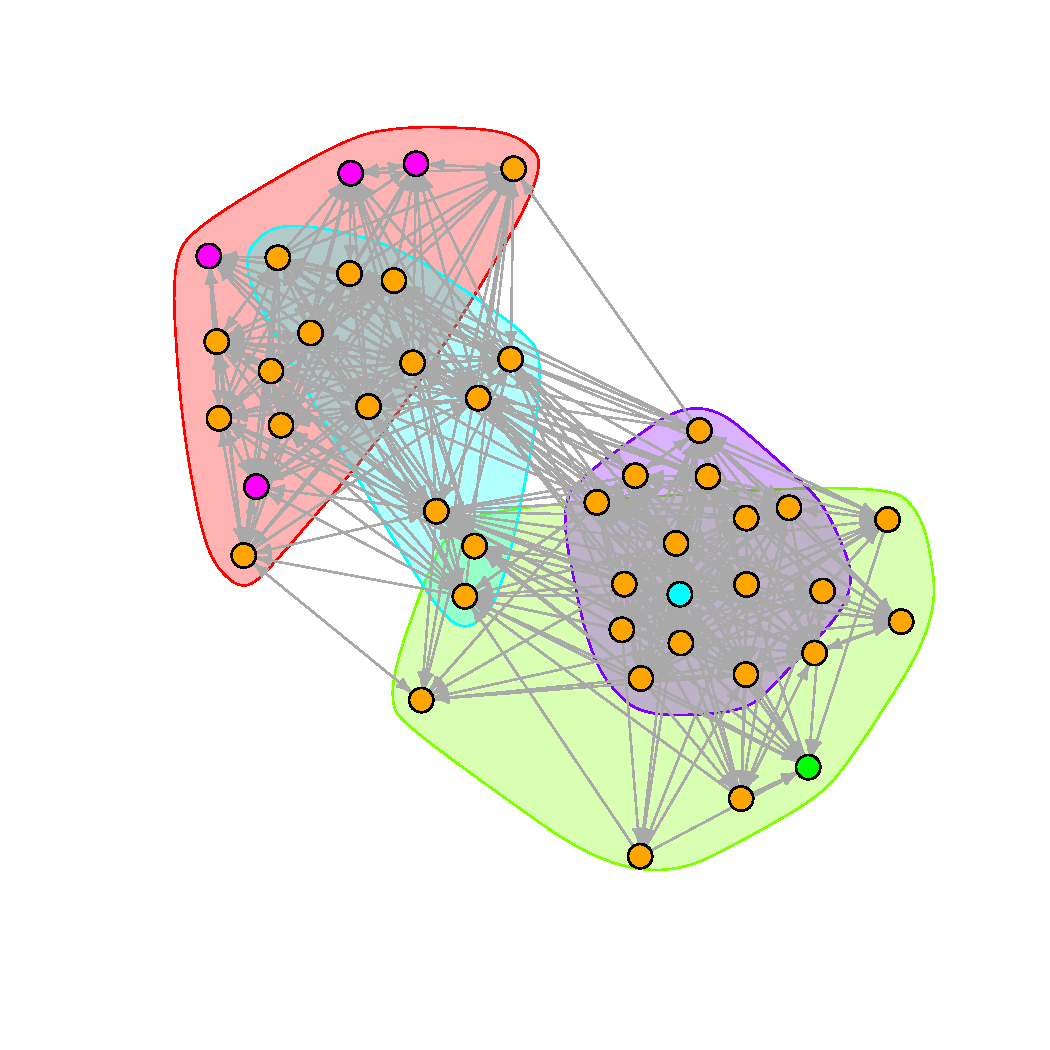
\includegraphics{gmmase_files/figure-latex/plotg-1.pdf}

This shows that we obtain the desired clustering!

\section[MNIST Data]{\texorpdfstring{MNIST Data\footnote{\url{http://yann.lecun.com/exdb/mnist/}}}{MNIST Data}}\label{mnist-data}

There are 42000 training images of 10 digits (from 0 to 9), and we
randomly select 1000 of them for our inference task.

\begin{Shaded}
\begin{Highlighting}[]
\KeywordTok{data}\NormalTok{(smnist)}
\NormalTok{slab <-}\StringTok{ }\NormalTok{smnist}\OperatorTok{$}\NormalTok{slab}
\NormalTok{strain <-}\StringTok{ }\NormalTok{smnist}\OperatorTok{$}\NormalTok{strain}
\NormalTok{(tab <-}\StringTok{ }\KeywordTok{table}\NormalTok{(slab))}
\end{Highlighting}
\end{Shaded}

\begin{verbatim}
## slab
##   0   1   2   3   4   5   6   7   8   9 
##  99 105 105 117  97  76  93 102  90 116
\end{verbatim}

\begin{Shaded}
\begin{Highlighting}[]
\NormalTok{numTrain <-}\StringTok{ }\KeywordTok{length}\NormalTok{(slab)}

\CommentTok{# Create a 28*28 matrix with pixel color values}
\NormalTok{res <-}\StringTok{ }\KeywordTok{sqrt}\NormalTok{(}\KeywordTok{ncol}\NormalTok{(strain))}
\NormalTok{glist <-}\StringTok{ }\KeywordTok{lapply}\NormalTok{(}\DecValTok{1}\OperatorTok{:}\NormalTok{numTrain, }\ControlFlowTok{function}\NormalTok{(x) }\KeywordTok{matrix}\NormalTok{(}\KeywordTok{unlist}\NormalTok{(strain[x,]),}\DataTypeTok{byrow=}\NormalTok{T,}\DataTypeTok{ncol=}\NormalTok{res))}
\end{Highlighting}
\end{Shaded}

The following shows five random slections of each digit from the sampled
data.

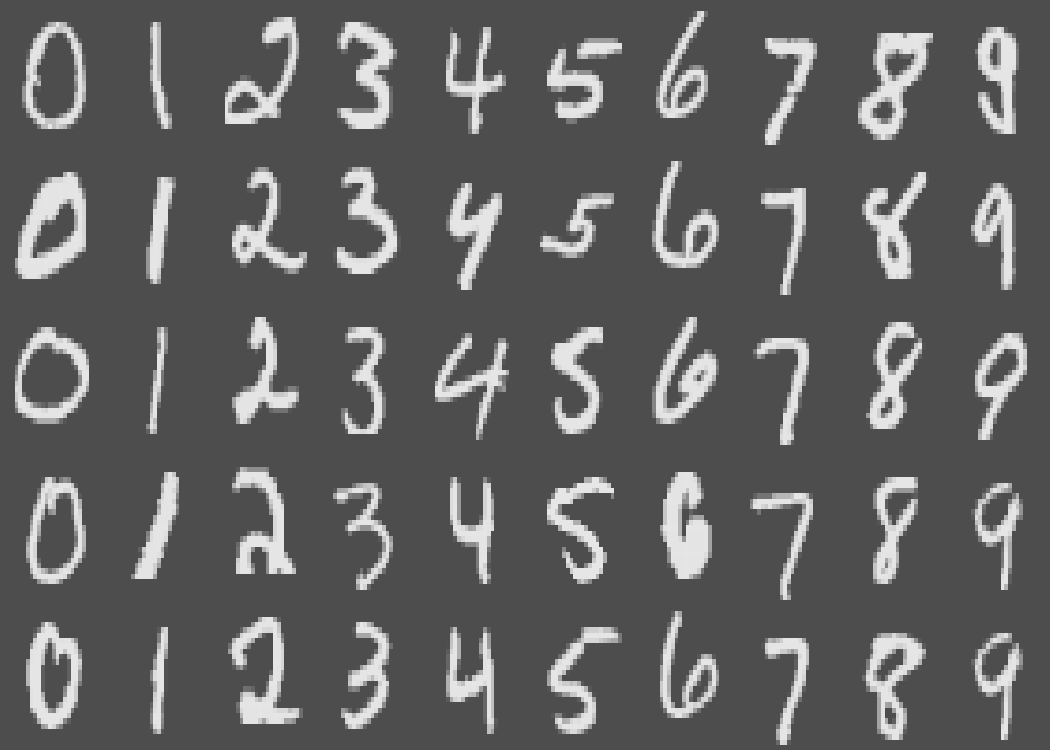
\includegraphics{gmmase_files/figure-latex/plotg3-1.pdf}

And, followings are averaged images of each digit from the sampled data.

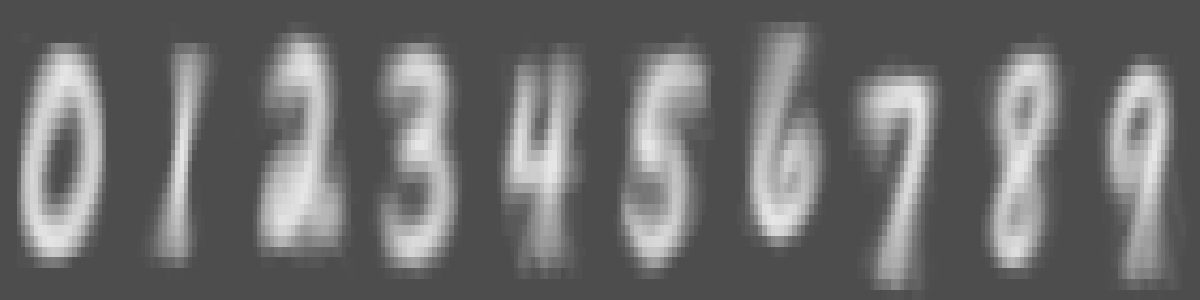
\includegraphics{gmmase_files/figure-latex/plotmean-1.pdf}

\subsection{Graph from Correlation
Coefficients}\label{graph-from-correlation-coefficients}

We use Pearson correlation coefficient between two images as a
similarity measure.

\begin{Shaded}
\begin{Highlighting}[]
\NormalTok{corrmat <-}\StringTok{ }\KeywordTok{calcCorr}\NormalTok{(}\KeywordTok{as.matrix}\NormalTok{(strain), }\DataTypeTok{useCorr=}\OtherTok{TRUE}\NormalTok{, }\DataTypeTok{recalc=}\OtherTok{TRUE}\NormalTok{); }\KeywordTok{range}\NormalTok{(corrmat)}
\end{Highlighting}
\end{Shaded}

\begin{verbatim}
# [1] -0.1241095  0.9777664
\end{verbatim}

\begin{Shaded}
\begin{Highlighting}[]
\CommentTok{#cor.eps <- median(as.vector(corrmat)); cat("threshold = ", cor.eps, "\textbackslash{}n")}
\NormalTok{cor.eps <-}\StringTok{ }\KeywordTok{quantile}\NormalTok{(}\KeywordTok{as.vector}\NormalTok{(corrmat),}\FloatTok{0.75}\NormalTok{); }\KeywordTok{cat}\NormalTok{(}\StringTok{"threshold = "}\NormalTok{, cor.eps, }\StringTok{"}\CharTok{\textbackslash{}n}\StringTok{"}\NormalTok{)}
\end{Highlighting}
\end{Shaded}

\begin{verbatim}
# threshold =  0.380978
\end{verbatim}

\begin{Shaded}
\begin{Highlighting}[]
\NormalTok{corrmat[corrmat}\OperatorTok{<}\NormalTok{cor.eps] <-}\StringTok{ }\DecValTok{0}
\NormalTok{g <-}\StringTok{ }\KeywordTok{graph.adjacency}\NormalTok{(}\KeywordTok{abs}\NormalTok{(corrmat), }\DataTypeTok{mode=}\StringTok{"undirected"}\NormalTok{, }\DataTypeTok{weighted=}\OtherTok{TRUE}\NormalTok{); }\KeywordTok{summary}\NormalTok{(g)}
\end{Highlighting}
\end{Shaded}

\begin{verbatim}
# IGRAPH 51fb0f2 U-W- 1000 125000 -- 
# + attr: weight (e/n)
\end{verbatim}

\begin{Shaded}
\begin{Highlighting}[]
\CommentTok{#library(RColorBrewer)}
\CommentTok{#rf <- colorRampPalette(rev(brewer.pal(11,'Spectral')))}
\CommentTok{#r <- rf(10)}
\CommentTok{#V(g)$color <- r[slab+1]}
\CommentTok{#plot(g, layout=layout.spring, }
\CommentTok{#     edge.arrow.size=0.5, vertex.label=NA, #vertex.label.cex=0.8, }
\CommentTok{#     vertex.size=3)#, vertex.color=rainbow(3, alpha=.5)[class])}


\NormalTok{out1 <-}\StringTok{ }\KeywordTok{gmmase}\NormalTok{(g, }\DataTypeTok{dmax =} \DecValTok{100}\NormalTok{, }\DataTypeTok{embed =} \StringTok{"ASE"}\NormalTok{, }\DataTypeTok{Kmax =} \DecValTok{10}\NormalTok{, }\DataTypeTok{clustering =} \StringTok{"GMM"}\NormalTok{, }\DataTypeTok{verbose=}\OtherTok{FALSE}\NormalTok{)}
\end{Highlighting}
\end{Shaded}

\begin{verbatim}
# 1. Finding an lcc...
# IGRAPH 387f265 U-W- 1000 125000 -- 
# + attr: weight (e/n)
# 2. Passing-to-rank...
# IGRAPH 387f265 U-W- 1000 125000 -- 
# + attr: weight (e/n)
# 3. Embedding the graph into dmax = 100...
# 4. Finding an elbow (dimension reduction)..., use dhat =  7 
# 5. Clustering vertices..., Khat =  10 
# ----------------------------------------------------
# Gaussian finite mixture model fitted by EM algorithm 
# ----------------------------------------------------
# 
# Mclust VVV (ellipsoidal, varying volume, shape, and orientation) model with 10 components:
# 
#  log.likelihood    n  df      BIC     ICL
#        1723.857 1000 359 967.8304 881.793
# 
# Clustering table:
#   1   2   3   4   5   6   7   8   9  10 
#  92 160  73  89 179 132  62 107  37  69
\end{verbatim}

\begin{Shaded}
\begin{Highlighting}[]
\CommentTok{#out1 <- gmmase(g, dmax = 100, embed = "LSE", Kmax = 10, clustering = "GMM", verbose=FALSE)}
\CommentTok{#out1 <- gmmase(g, dmax = 100, embed = "ASE", Kmax = 10, clustering = "Kmeans", verbose=FALSE)}

\NormalTok{Xhat1 <-}\StringTok{ }\NormalTok{out1}\OperatorTok{$}\NormalTok{mc}\OperatorTok{$}\NormalTok{data}
\NormalTok{Yhat <-}\StringTok{ }\NormalTok{out1}\OperatorTok{$}\NormalTok{Y}
\NormalTok{df2 <-}\StringTok{ }\KeywordTok{data.frame}\NormalTok{(}\DataTypeTok{Xhat=}\NormalTok{Xhat1, }\DataTypeTok{lab=}\KeywordTok{as.factor}\NormalTok{(slab), }\DataTypeTok{cluster=}\KeywordTok{as.factor}\NormalTok{(Yhat))}
\KeywordTok{ggpairs}\NormalTok{(df2, }\DataTypeTok{columns=}\DecValTok{1}\OperatorTok{:}\NormalTok{(}\KeywordTok{ncol}\NormalTok{(df2)}\OperatorTok{-}\DecValTok{2}\NormalTok{), }\DataTypeTok{mapping=}\KeywordTok{aes}\NormalTok{(}\DataTypeTok{color=}\NormalTok{cluster, }\DataTypeTok{shape=}\NormalTok{lab, }\DataTypeTok{alpha=}\FloatTok{0.5}\NormalTok{))}
\end{Highlighting}
\end{Shaded}

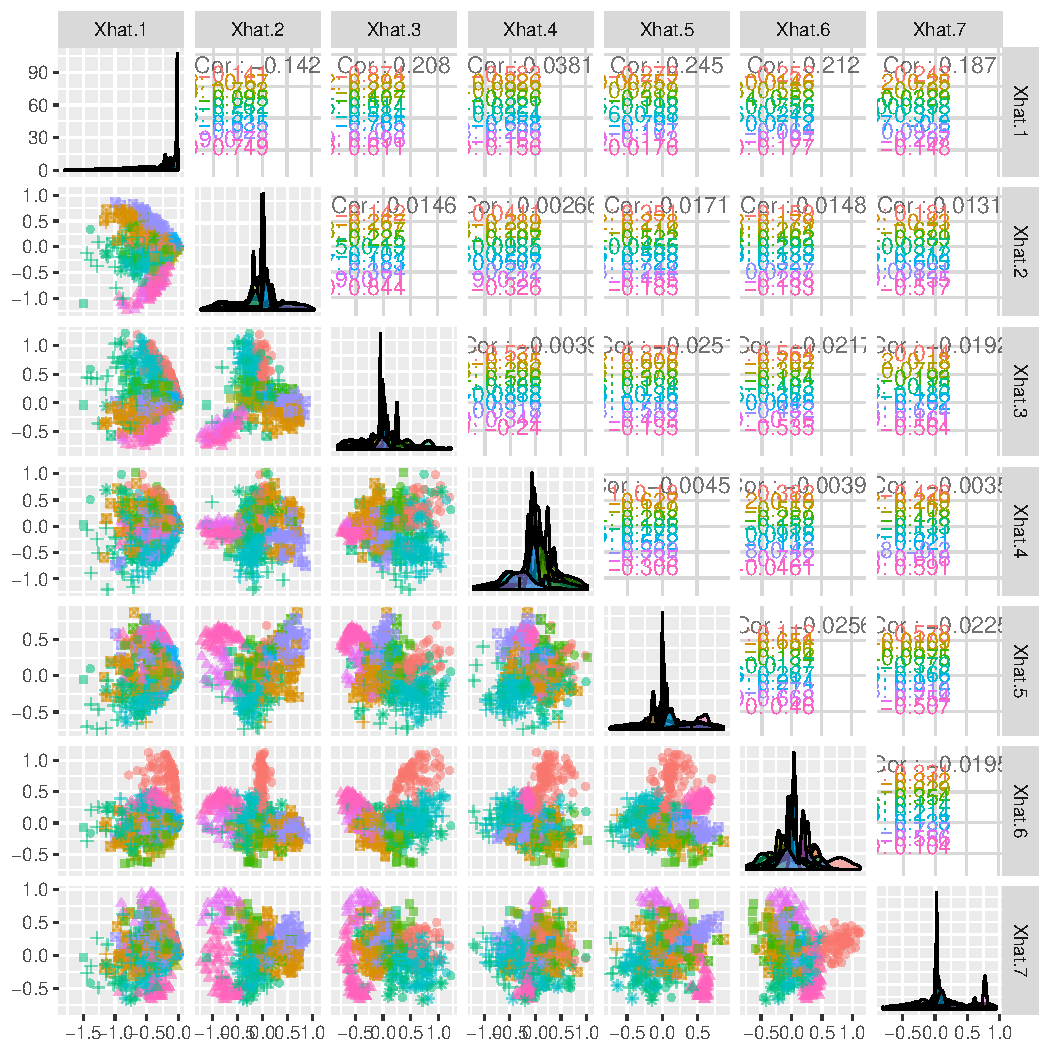
\includegraphics{gmmase_files/figure-latex/cor-1.pdf}

Now we plot nine random images of the cluster that contains each digist
the most.

\begin{longtable}[]{@{}lrrrrrrrrrr@{}}
\toprule
& 1 & 2 & 3 & 4 & 5 & 6 & 7 & 8 & 9 & 10\tabularnewline
\midrule
\endhead
0 & 82 & 0 & 0 & 1 & 8 & 6 & 2 & 0 & 0 & 0\tabularnewline
1 & 0 & 0 & 4 & 0 & 1 & 0 & 0 & 0 & 33 & 67\tabularnewline
2 & 1 & 6 & 45 & 23 & 11 & 3 & 15 & 1 & 0 & 0\tabularnewline
3 & 1 & 5 & 1 & 1 & 28 & 76 & 4 & 1 & 0 & 0\tabularnewline
4 & 0 & 45 & 1 & 4 & 3 & 0 & 7 & 37 & 0 & 0\tabularnewline
5 & 5 & 2 & 12 & 2 & 12 & 36 & 3 & 4 & 0 & 0\tabularnewline
6 & 2 & 0 & 3 & 55 & 15 & 0 & 17 & 1 & 0 & 0\tabularnewline
7 & 0 & 50 & 3 & 0 & 13 & 0 & 7 & 25 & 4 & 0\tabularnewline
8 & 0 & 8 & 4 & 0 & 66 & 11 & 0 & 0 & 0 & 1\tabularnewline
9 & 1 & 44 & 0 & 3 & 22 & 0 & 7 & 38 & 0 & 1\tabularnewline
\bottomrule
\end{longtable}

\begin{verbatim}
# ARI for Khat = 10  is  0.31
\end{verbatim}

\begin{verbatim}
#  0  1  2  3  4  5  6  7  8  9 
#  1 10  3  6  2  6  4  2  5  2
\end{verbatim}

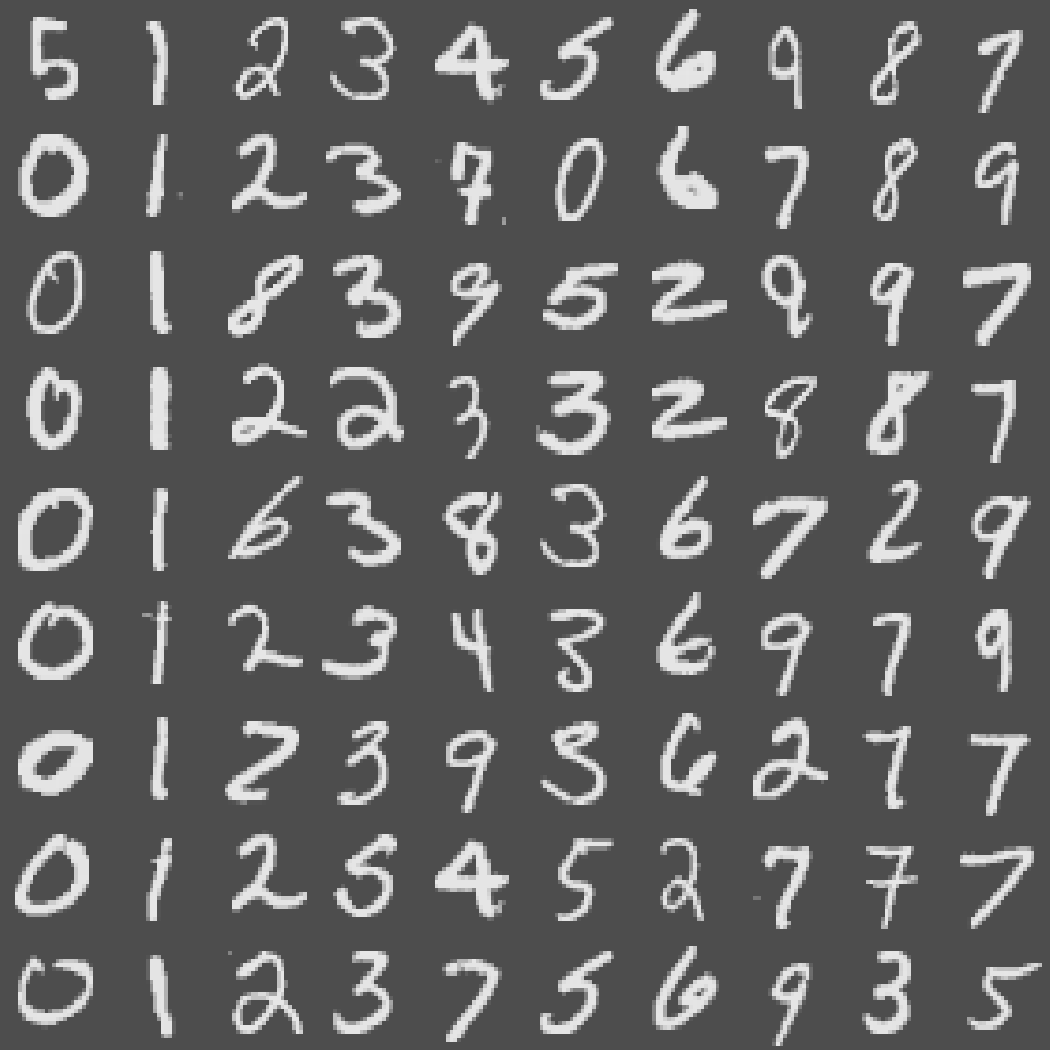
\includegraphics{gmmase_files/figure-latex/mnistplot-1.pdf}

\subsection{\texorpdfstring{Graph from \(k\)-nearest
neighbors}{Graph from k-nearest neighbors}}\label{graph-from-k-nearest-neighbors}

From a given point \(i\), it is connected to the \(k\) other points that
are closest to it in the Euclidean space.

\begin{Shaded}
\begin{Highlighting}[]
\NormalTok{D <-}\StringTok{ }\KeywordTok{as.matrix}\NormalTok{(}\KeywordTok{dist}\NormalTok{(strain))}
\NormalTok{kvec <-}\StringTok{ }\DecValTok{3}\OperatorTok{:}\DecValTok{9}
\NormalTok{ariv <-}\StringTok{ }\NormalTok{dhatv <-}\StringTok{ }\NormalTok{khatv <-}\StringTok{ }\KeywordTok{rep}\NormalTok{(}\DecValTok{0}\NormalTok{,}\KeywordTok{length}\NormalTok{(kvec))}
\ControlFlowTok{for}\NormalTok{ (k }\ControlFlowTok{in} \DecValTok{1}\OperatorTok{:}\KeywordTok{length}\NormalTok{(kvec)) \{}
\NormalTok{    A <-}\StringTok{ }\KeywordTok{matrix}\NormalTok{(}\DecValTok{0}\NormalTok{,numTrain,numTrain)}
    \ControlFlowTok{for}\NormalTok{ (i }\ControlFlowTok{in} \DecValTok{1}\OperatorTok{:}\NormalTok{numTrain) \{}
\NormalTok{        nn <-}\StringTok{ }\KeywordTok{order}\NormalTok{(D[i,])[}\DecValTok{1}\OperatorTok{:}\NormalTok{kvec[k]]}
\NormalTok{        A[i,nn] <-}\StringTok{ }\NormalTok{A[nn,i] <-}\StringTok{ }\DecValTok{1}
\NormalTok{    \}}
    \KeywordTok{diag}\NormalTok{(A) <-}\StringTok{ }\DecValTok{0}

\NormalTok{    g.knn <-}\StringTok{ }\KeywordTok{graph.adjacency}\NormalTok{(A, }\DataTypeTok{mode=}\StringTok{"undirected"}\NormalTok{); }\KeywordTok{summary}\NormalTok{(g.knn)}
\NormalTok{    out2 <-}\StringTok{ }\KeywordTok{gmmase}\NormalTok{(g.knn, }\DataTypeTok{dmax =} \DecValTok{20}\NormalTok{, }\DataTypeTok{embed =} \StringTok{"ASE"}\NormalTok{, }\DataTypeTok{Kmax =} \DecValTok{10}\NormalTok{, }\DataTypeTok{clustering =} \StringTok{"GMM"}\NormalTok{,}
                   \DataTypeTok{verbose=}\OtherTok{FALSE}\NormalTok{, }\DataTypeTok{doplot=}\OtherTok{FALSE}\NormalTok{)}
\NormalTok{    dhatv[k] <-}\StringTok{ }\NormalTok{out2}\OperatorTok{$}\NormalTok{elb}
\NormalTok{    Yhat2 <-}\StringTok{ }\NormalTok{out2}\OperatorTok{$}\NormalTok{Y}
\NormalTok{    khatv[k] <-}\StringTok{ }\KeywordTok{max}\NormalTok{(Yhat2)}
\NormalTok{    ariv[k] <-}\StringTok{ }\KeywordTok{adjustedRandIndex}\NormalTok{(slab, Yhat2)}
    \KeywordTok{cat}\NormalTok{(}\StringTok{"k = "}\NormalTok{, kvec[k], }\StringTok{", dhat = "}\NormalTok{, dhatv[k], }\StringTok{", Khat = "}\NormalTok{, khatv[k], }\StringTok{", ari = "}\NormalTok{, ariv[k], }\StringTok{"}\CharTok{\textbackslash{}n}\StringTok{"}\NormalTok{)}
\NormalTok{\}}
\end{Highlighting}
\end{Shaded}

\begin{longtable}[]{@{}rrrr@{}}
\toprule
k & dhat & khat & ari\tabularnewline
\midrule
\endhead
3 & 17 & 10 & 0.24\tabularnewline
4 & 8 & 10 & 0.27\tabularnewline
5 & 7 & 10 & 0.27\tabularnewline
6 & 10 & 10 & 0.36\tabularnewline
7 & 9 & 10 & 0.40\tabularnewline
8 & 9 & 10 & 0.38\tabularnewline
9 & 10 & 10 & 0.42\tabularnewline
\bottomrule
\end{longtable}

Let's see the example run of \$argmax\_k ARI = \$ 9.

\begin{verbatim}
# IGRAPH 47a08fb U--- 1000 5797 --
\end{verbatim}

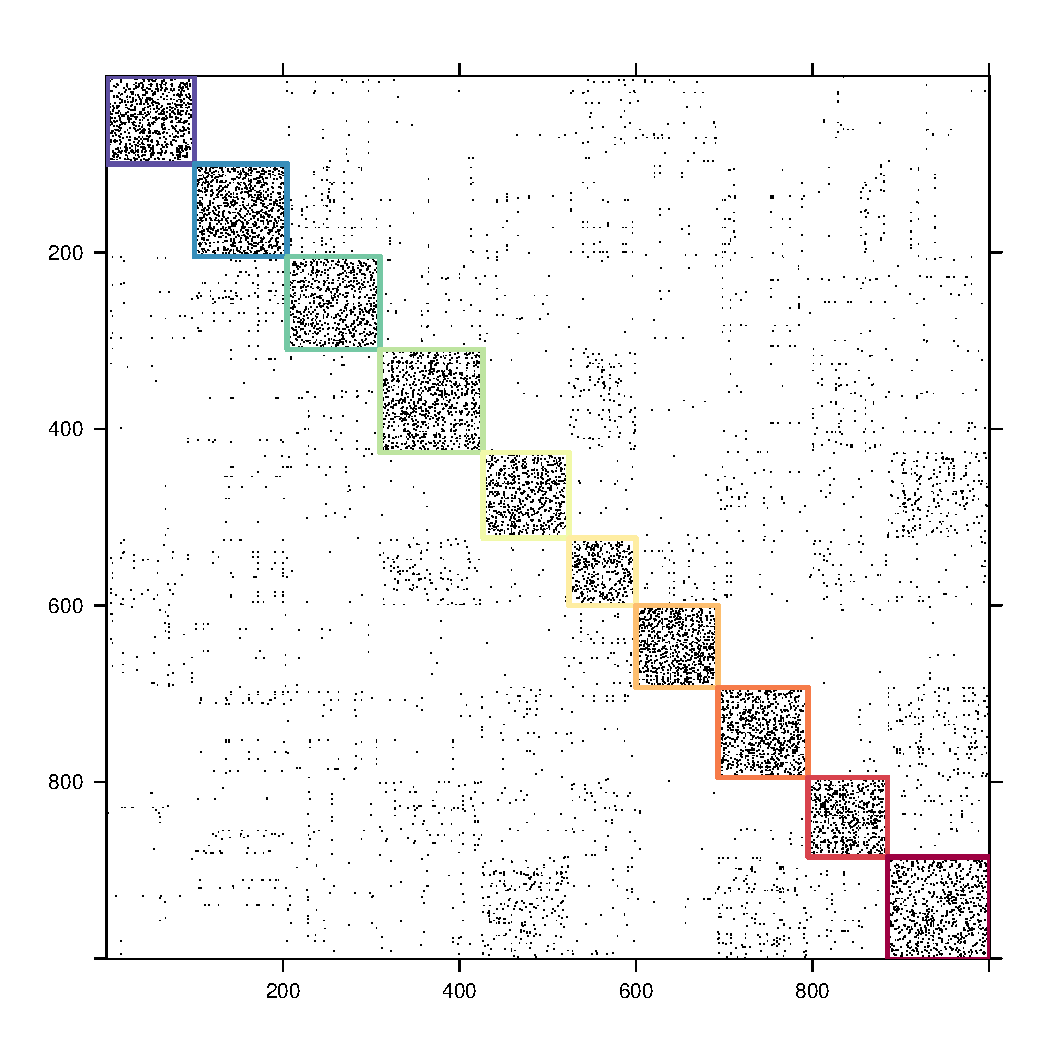
\includegraphics{gmmase_files/figure-latex/knnplot-1.pdf}
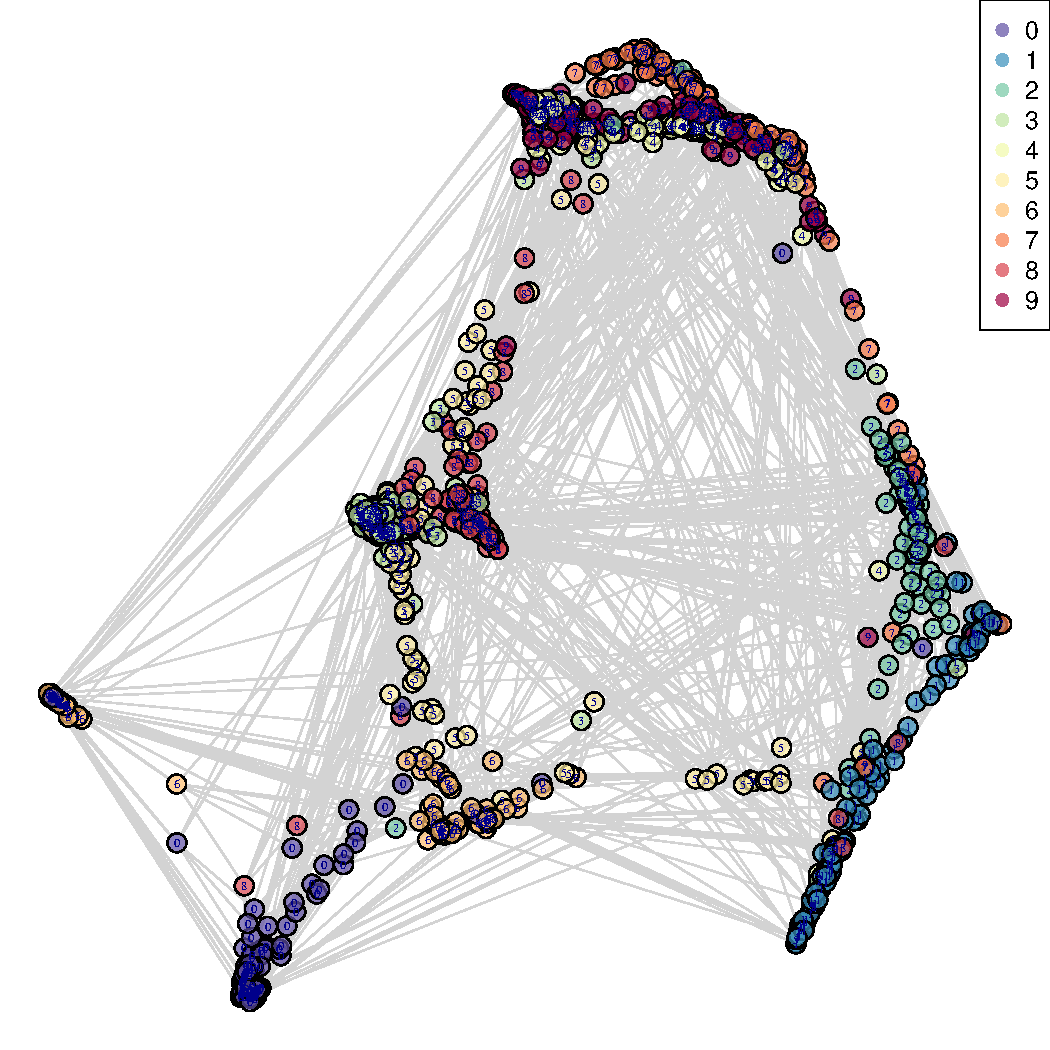
\includegraphics{gmmase_files/figure-latex/knnplot-2.pdf}

\begin{verbatim}
# 1. Finding an lcc...
# IGRAPH 46575c3 U--- 1000 5797 -- 
# + attr: color (v/c)
# 3. Embedding the graph into dmax = 20...
# 4. Finding an elbow (dimension reduction)..., use dhat =  10 
# 5. Clustering vertices..., Khat =  10 
# ----------------------------------------------------
# Gaussian finite mixture model fitted by EM algorithm 
# ----------------------------------------------------
# 
# Mclust VVV (ellipsoidal, varying volume, shape, and orientation) model with 10 components:
# 
#  log.likelihood    n  df      BIC      ICL
#        27414.33 1000 659 50276.46 50252.37
# 
# Clustering table:
#   1   2   3   4   5   6   7   8   9  10 
# 164 100 103  75  84  81  88  98  83 124
\end{verbatim}

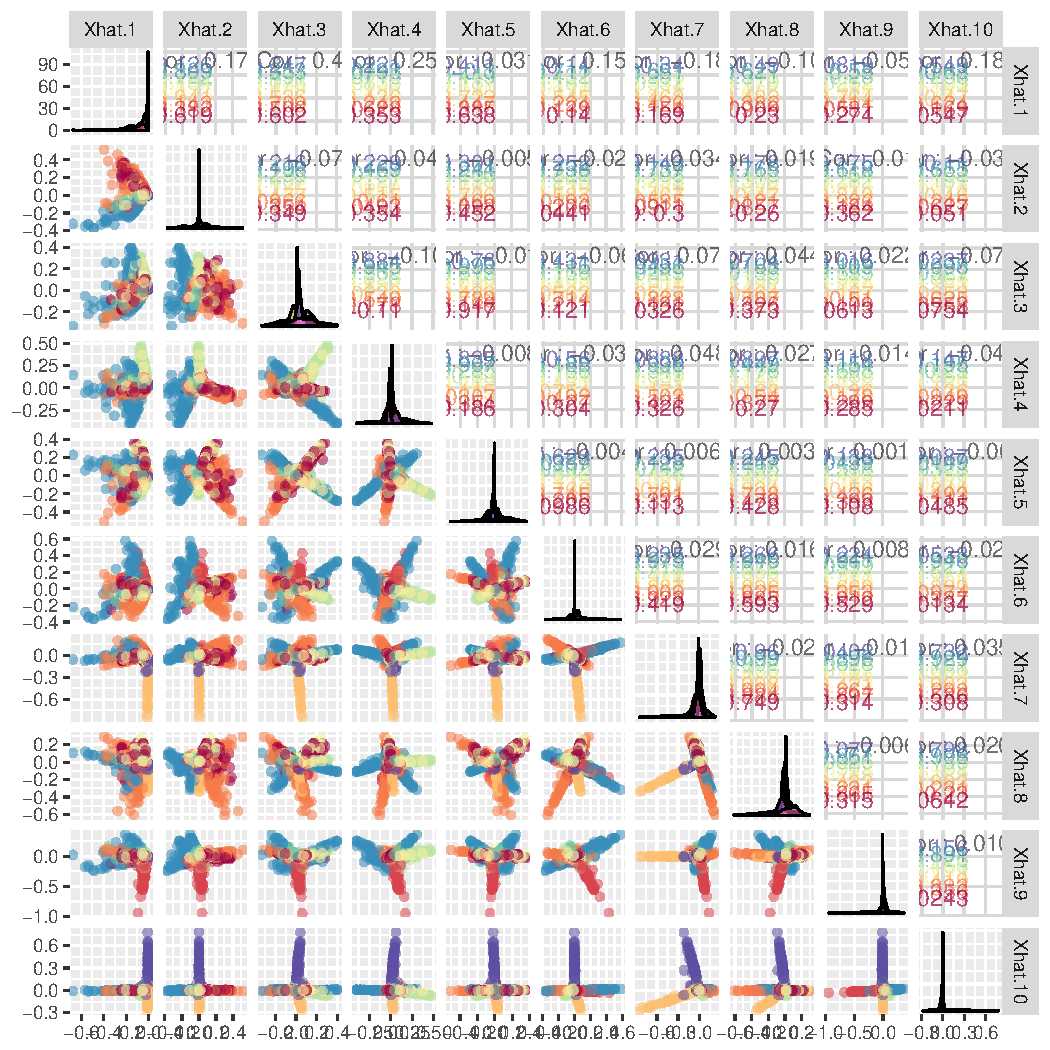
\includegraphics{gmmase_files/figure-latex/knnplot-3.pdf}

\begin{longtable}[]{@{}lrrrrrrrrrr@{}}
\toprule
& 1 & 2 & 3 & 4 & 5 & 6 & 7 & 8 & 9 & 10\tabularnewline
\midrule
\endhead
0 & 0 & 0 & 6 & 74 & 0 & 0 & 19 & 0 & 0 & 0\tabularnewline
1 & 105 & 0 & 0 & 0 & 0 & 0 & 0 & 0 & 0 & 0\tabularnewline
2 & 24 & 0 & 5 & 0 & 5 & 20 & 4 & 1 & 0 & 46\tabularnewline
3 & 3 & 0 & 0 & 0 & 11 & 5 & 21 & 75 & 0 & 2\tabularnewline
4 & 3 & 9 & 1 & 0 & 1 & 32 & 0 & 0 & 39 & 12\tabularnewline
5 & 10 & 1 & 2 & 0 & 1 & 8 & 31 & 19 & 0 & 4\tabularnewline
6 & 4 & 0 & 87 & 0 & 0 & 0 & 2 & 0 & 0 & 0\tabularnewline
7 & 7 & 53 & 0 & 0 & 0 & 1 & 0 & 0 & 2 & 39\tabularnewline
8 & 5 & 2 & 0 & 1 & 66 & 3 & 9 & 3 & 0 & 1\tabularnewline
9 & 3 & 35 & 2 & 0 & 0 & 12 & 2 & 0 & 42 & 20\tabularnewline
\bottomrule
\end{longtable}

\begin{verbatim}
# ARI for Khat = 10  is  0.42
\end{verbatim}

\begin{verbatim}
#  0  1  2  3  4  5  6  7  8  9 
#  4  1 10  8  9  7  3  2  5  9
\end{verbatim}

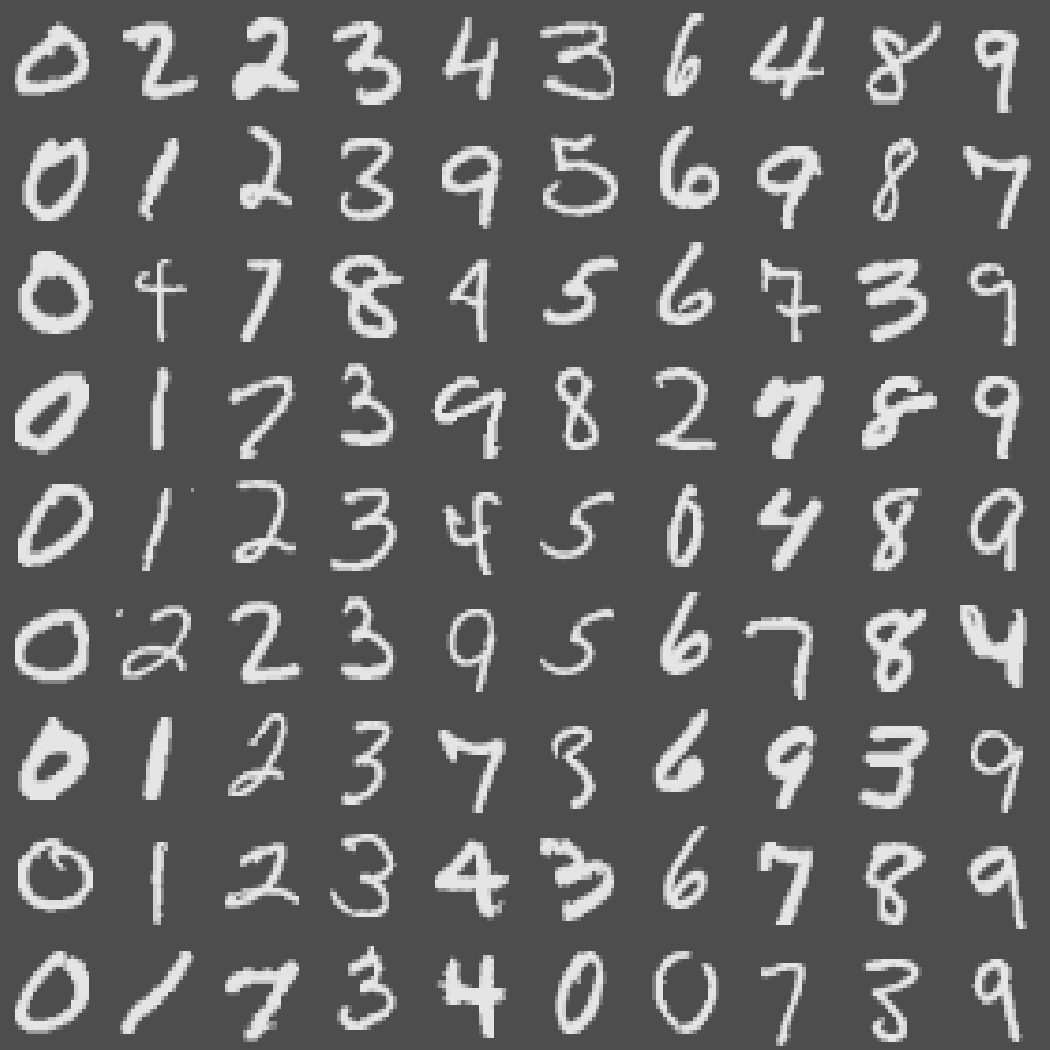
\includegraphics{gmmase_files/figure-latex/knnplot-4.pdf}


\end{document}
